\chapter{课题的来源背景以及研究意义}
\section{课题来源}

课题来源于。。。。。拟针对绳索驱动的新型超冗余连续型柔性臂在复杂工作环境下进行探测等任务,进行系统的运动学建模,样机的设计及调试,并进一步研究探索针对此类柔性臂的运动学规划及避障算法。
\section{研究背景及意义}

随着经济的发展和社会的进步,机器人的应用领域不断拓展,应用环境也愈发复杂。以工业机器人为代表的传统刚性机械臂在结构化的工作环境下的程序化操作得到了广泛应用,但刚性机械臂在非结构环境(例如废墟、复杂管道等)下的局限性正日益显露。在传统工业机器人中,电机、传动机构等被放置于关节臂杆中,不仅增大了关节的质量,还加大了关节尺寸;另外,受制于质量和体积的限制,具有长而粗臂杆的这类刚性机械臂的自由度往往较少,其运动的灵活性进一步恶化,难以完成狭小环境下的各类作业要求。为了解决传统机器人在复杂环境下操作所面临的问题,许多研究人员将目光投向了具有更多运动自由度更好弯曲特性的连续型机器人的研究中。

连续型机械臂受自然界中象鼻等生物体结构启发,一般由弹性物体作为支撑,将许多模块化关节串联而成,或者直接用完整无间断的弹性材料作为机械臂本体,因而具有超高冗余度甚至理论上无限多自由度。这种结构形式使得连续型机械臂具有良好的运动灵活性和柔顺性,因而特别适合于狭小空间下的避障作业。图\ref{fig:compare_tra_con}显示了传统刚性臂与连续型机械臂在狭小环境中作业能力的差异。可以看出,具有超高冗余度的连续型机械臂具有更好的弯曲特性和障碍穿越能力。
\begin{figure}[!htbp]
	\centering
	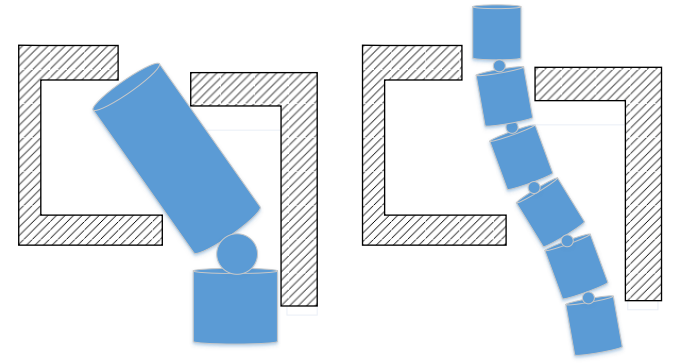
\includegraphics[width=.75\textwidth]{figures/compare_tra_con.png}
	\caption{传统刚性机械臂与连续型机械臂在狭小空间中的作业能力对比}
	\label{fig:compare_tra_con}
\end{figure}

连续型柔性臂的灵活性、柔顺性使得其在非结构复杂环境中具有广阔的应用前景。在航空航天领域中,连续型柔性臂可以穿越航天器的桁架结构和组件间隙,深入到结构内部进行探测、在轨维修等任务\cite{xu_modified_2017};在工业生产领域,可以通过孔洞等深入结构内部进行钻孔、焊接等工作(如图\ref{fig:app_airplane}和图\ref{fig:app_pipeline});在危险环境中,可以进入到狭小缝隙中进行结构的探伤和检修(如图\ref{fig:app_nuclear});可用于地震后废墟内生命迹象检测(如图\ref{fig:app_debri});还可用于外科手术中对体内空腔结构的检查和微创手术等(如图\ref{fig:app_surgery})。
\begin{figure}[h]
	\centering%
	\subcaptionbox{飞机舱内钻孔\label{fig:app_airplane}}
	{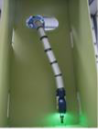
\includegraphics[height=4cm]{figures/app_airplane.png}}%
	\hspace{1em}%
	\subcaptionbox{复杂管道中焊接\label{fig:app_pipeline}}
	{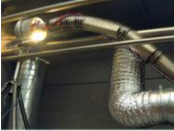
\includegraphics[height=4cm]{figures/app_pipeline.png}}
	\hspace{1em}%
	\subcaptionbox{核电站设备检修\label{fig:app_nuclear}}
	{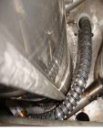
\includegraphics[height=4cm]{figures/app_nuclear.png}}
	\\
	\vspace{1em}
	\subcaptionbox{地震灾害救援\label{fig:app_debri}}
	{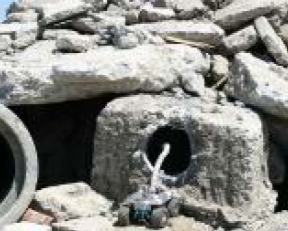
\includegraphics[height=4cm]{figures/app_debri.png}}
	\hspace{1em}%
	\subcaptionbox{外科手术\label{fig:app_surgery}}
	{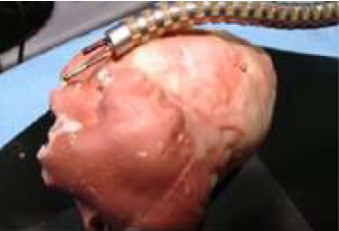
\includegraphics[height=4cm]{figures/app_surgery.png}}
	\caption{连续型机械臂在各种复杂环境中的应用}
	\label{fig:apps}
\end{figure}

从驱动方式上看,连续型机器人可分为腱驱动式、同心圆管式和其他新型机构驱动等三类。绳索作为腱的一种,采用其作为驱动传动机构,具有以下优点:首先,通过柔性绳索传动,原本位于关节连接处的电机、控制电路、减速装置等可以迁移到根部基座上,实现驱动机构和执行机构的分离,从而使得电机控制电路等远离外界复杂环境的不利影响,并且能够显著减小机械臂的体积和质量;其次,关节质量和体积的减小意味着在整体质量和体积的约束下,机械臂可以增加更多的关节模块,从而使得机械臂具有更多的运动自由度,也就具有更强的运动灵活性和避障能力;再者,绳索驱动的连续型机械臂相比于其他种类的连续型机器人,对材料工艺等要求较低,结构也比较简单,更容易进行原理样机的设计和制作。

综上所述,为了应对新的复杂环境对机器人提出的新挑战,有必要对连续型机器人展开研究,采用绳索驱动,可以减小机械臂重量和体积,组装具有超冗余度的柔性臂,并探索其在非结构环境中运动规划方法。

